\documentclass[../main.tex]{subfiles}
\graphicspath{{\subfix{../figures/}}}
%
\begin{document}
\section{模板方法模式(Template Method)}
模板方法模式是最为常见的几个模式之一。模板方法模式是基于继承的代码复用的基本技术,模板方法模式的结构和用法也是面向对象设计的核心。
模板方法模式为设计抽象类和实现具体子类的设计师之间的协作提供了可能:一个设计师负责给出一个算法的轮廓和骨架,另一些设计师则负责实现这个算法的各个逻辑步骤。

模板方法所代表的行为称为顶级行为,其逻辑称为顶级逻辑。模板方法模式的简略类图如下图所示。
%
\begin{figure}[H]
  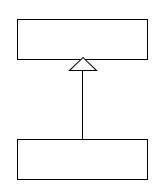
\includegraphics[width=0.20\textwidth]{28_1.jpg}
\end{figure}
%
模板方法模式的静态结构如下图所示:
%
\begin{figure}[H]
  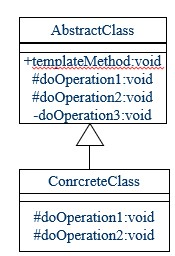
\includegraphics[width=0.20\textwidth]{28_2.jpg}
\end{figure}
%
\lstinputlisting[language=java]{./code/28/1/AbstractClass.java}
\lstinputlisting[language=java]{./code/28/1/ConcreteClass.java}
%
\subsection{好莱坞原则}
在好莱坞工作的演艺界人士都了解,在把简历递交给好莱坞的娱乐公司以后,所能做的就是等待。这些公司会告诉他们“不要给我们打电话,我们会给你打”。这便是所谓的“好莱坞原则”。好莱坞原则的关键之处,是娱乐公司对娱乐项目的完全控制。应聘的演员只是被动地服从总项目流程的安排,在需要的时候完成流程中的具体环节。
虽然“好莱坞原则”很早的时候在不同的题材里被讨论过,使用这个比喻描写模板方法模式则是由【GoF】给出的,他们认为“好莱坞原则”体现了模板。

\textbf{模式的关键}:
子类可以置换掉父类的可变部分,但是子类却不可以改变模板方法所定义的顶层逻辑。
每当定义一个新的子类时,不要按照控制流程的思路去设计其职责,而应当按照“责任”的思路去设计。换言之,应当考虑有哪些操作是必须置换掉的,哪些操作是可以置换掉的,以及那些操作是不可以置换掉的。使用模板方法模式可以使这些责任变的清晰。
%
\subsection{例:计算账户利息}
\lstinputlisting[language=java]{./code/28/2/Account.java}
\lstinputlisting[language=java]{./code/28/2/MoneyMarketAccount.java}
\lstinputlisting[language=java]{./code/28/2/CDAccount.java}
\lstinputlisting[language=java]{./code/28/2/Client.java}
%
\textbf{运行结果}:
%
\begin{itemize}
  \item Interested from Money Market account 325.935
  \item Interested from CD account 470.795
\end{itemize}
%
显然,货币市场帐户和定期存款帐户的不同利息数额,是由于基本方法在不同的具体子类中有不同的实现所造成。
%
\subsection{模板方法模式中的方法}
\begin{itemize}
  \item \textbf{模板方法}:
    一个模板方法是定义在抽象类中的,把基本操作方法组合在一起形成一个总算法或一个总行为的方法。这个模板方法一般会在抽象类中定义,并由子类不加以修改地完全继承下来。
    一个抽象类可以有任意多个模板方法,而不限于一个。每一个模板方法都可以调用任意多个具体方法。
  \item \textbf{基本方法}有可以分为三种:抽象方法、具体方法、钩子/回调方法.
\end{itemize}
%
\begin{figure}[H]
  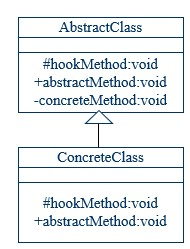
\includegraphics[width=0.20\textwidth]{28_3.jpg}
\end{figure}
%
\subsection{应用:代码重构}
\begin{itemize}
  \item 模板方法模式可以作为方法层次上的代码重构的一个重要手段。
  \item 不良的代码设计常常会将过多的代码放在一个方法里面,造成一个具有几千行代码的大方法。这样的方法应当拆分成一些较小的方法,拆分的策略往往可以使用模板方法模式。
  \item 将大方法打破
\end{itemize}
%
假设下面就是这个需要重构的过大的方法:
%
\lstinputlisting[language=java]{./code/28/3/1.java}
%
\lstinputlisting[language=java]{./code/28/3/2.java}
%
划分后的类图如下图所示。
\begin{figure}[H]
  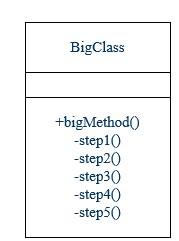
\includegraphics[width=0.20\textwidth]{28_4.jpg}
\end{figure}
%
\textbf{以多态性取代条件转移}:
以下代码说明其三个方法作为一个新方法newMethod()的多态性体现,划分到三个不同的子类中去.
%
\lstinputlisting[language=java]{./code/28/3/3.java}
%
下图所示是代码重构后的最终结果。
%
\begin{figure}[H]
  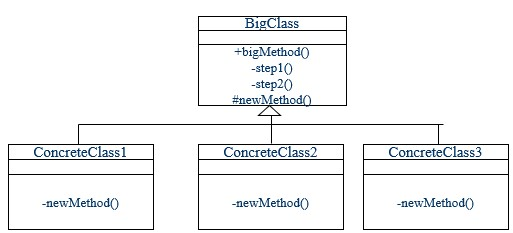
\includegraphics[width=0.55\textwidth]{28_5.jpg}
\end{figure}
%
\end{document}
